\documentclass{article}

\usepackage{fancyhdr, lastpage}
\usepackage[inline]{enumitem}
\usepackage{listings}
\usepackage[scaled=0.95]{inconsolata}  % Use a monospaced font, like Inconsolata
\usepackage{wasysym}
\usepackage{booktabs}
\usepackage{booktabs, multicol, multirow, array, threeparttable}
\usepackage{siunitx}
\usepackage{xfrac}
\usepackage{extramarks}
\usepackage{amsmath, amsthm, amsfonts, mathtools, empheq}
\usepackage{caption}
\usepackage[table]{xcolor}
\usepackage{tikz}
\usepackage[most]{tcolorbox}
\usepackage{pagecolor} %% for dark background
\usepackage{hyperref}
\usepackage{refcount}
\usepackage{subfigure}

\topmargin=-0.45in
\evensidemargin=0in
\oddsidemargin=0in
\textwidth=6.5in
\textheight=9.0in
\headsep=0.25in

\linespread{1.1}

% Define a command to print last page number without hyperlink
\newcommand*{\lastpagewithoutlink}{%
    \getpagerefnumber{LastPage}%
}

\pagestyle{fancy}
\lhead{\hmwkAuthorName}
\chead{\hmwkTitle}
\rhead{\hmwkClass}
\lfoot{\lastxmark}
\cfoot{Page \thepage \ of \lastpagewithoutlink}


\renewcommand\headrulewidth{0.4pt}
\renewcommand\footrulewidth{0.4pt}

\setlength\parindent{0pt}

%
% Create Problem Sections
%

\newcommand{\enterProblemHeader}[1]{
    \nobreak\extramarks{}{Problem \arabic{#1} continued on next page\ldots}\nobreak{}
    \nobreak\extramarks{Problem \arabic{#1} (continued)}{Problem \arabic{#1} continued on next page\ldots}\nobreak{}
}

\newcommand{\exitProblemHeader}[1]{
    \nobreak\extramarks{Problem \arabic{#1} (continued)}{Problem \arabic{#1} continued on next page\ldots}\nobreak{}
    \stepcounter{#1}
    \nobreak\extramarks{Problem \arabic{#1}}{}\nobreak{}
}

\setcounter{secnumdepth}{0}
\newcounter{partCounter}
\newcounter{homeworkProblemCounter}
\setcounter{homeworkProblemCounter}{1}
\nobreak\extramarks{Problem \arabic{homeworkProblemCounter}}{}\nobreak{}

%
% Homework Problem Environment
%
% This environment takes an optional argument. When given, it will adjust the
% problem counter. This is useful for when the problems given for your
% assignment aren't sequential. See the last 3 problems of this template for an
% example.
%
\newenvironment{homeworkProblem}[1][-1]{
    \ifnum#1>0
        \setcounter{homeworkProblemCounter}{#1}
    \fi
    \section{Problem \arabic{homeworkProblemCounter}}
    \setcounter{partCounter}{1}
    \enterProblemHeader{homeworkProblemCounter}
}{
    \exitProblemHeader{homeworkProblemCounter}
}

%
% Homework Details
%   - Title
%   - Due date
%   - Class
%   - Section/Time
%   - Instructor
%   - Author
%

\newcommand{\hmwkTitle}{Homework\ \#4}
\newcommand{\hmwkDueDate}{April 20, 2024}
\newcommand{\hmwkClass}{EGR 5110}
\newcommand{\hmwkClassTime}{}
\newcommand{\hmwkClassInstructor}{Professor Nissenson}
\newcommand{\hmwkAuthorName}{\textbf{Francisco Sanudo}}

%
% Title Page
%

\title{
    \vspace{2in}
    \textmd{\textbf{\hmwkClass:\ \hmwkTitle}}\\
    \normalsize\vspace{0.1in}\small{Due\ on\ \hmwkDueDate\ at 11:59pm}\\
    \vspace{0.1in}\large{\textit{\hmwkClassInstructor\ \hmwkClassTime}}
    \vspace{3in}
}

\author{\hmwkAuthorName}
\date{}

\renewcommand{\part}[1]{\textbf{\large Part \Alph{partCounter}}\stepcounter{partCounter}\\}

%
% More settings
%

% Table Settings
% \setlength{\tabcolsep}{5pt} % Gap before text starts
\renewcommand{\arraystretch}{2.5} % Cell Height Scaling
\setlength{\arrayrulewidth}{0.5mm} % Table Border Thickness
\arrayrulecolor{blue} % Table Border Color
\newcolumntype{s}{>{\columncolor{black!10}} c}

% Link Settings
\hypersetup{
    colorlinks=false,       % false: boxed links; true: colored links
    linkcolor=red,          % color of internal links (change box color with linkbordercolor)
    citecolor=green,        % color of links to bibliography
    urlcolor=cyan,           % color of external links
    pdftitle={EGR 5110 HW3}
}

% Color defintions
\definecolor{magenta}{RGB}{255,0,255}
\definecolor{cyan}{RGB}{0,255,255}
\definecolor{white}{RGB}{255,255,255}
\definecolor{red}{RGB}{255,0,0}
\definecolor{green}{RGB}{0,255,0}
\definecolor{orange}{RGB}{255,165,0}
\definecolor{yellow}{RGB}{255,255,0}
\definecolor{blue}{RGB}{10,10,255}

% Text color shortcuts
\newcommand{\cw}{\color{white}}
\newcommand{\cm}{\color{magenta}}
\newcommand{\cc}{\color{cyan}}
\newcommand{\cred}{\color{red}}
\newcommand{\cb}{\color{blue}}
\newcommand{\cg}{\color{green}}
\newcommand{\cy}{\color{yellow}}
\newcommand{\co}{\color{orange}}

%
% Various Helper Commands
%


% For derivatives
\newcommand{\deriv}[2]{\frac{d#1}{d#2}}

% For partial derivatives
\newcommand{\pderiv}[2]{\displaystyle \frac{\partial #1}{\partial #2}}

% Redefine \dfrac if you want all fractions to be in display style automatically
\newcommand{\ddfrac}[2]{\frac{\displaystyle #1}{\displaystyle #2}}

% Alias for the Solution section header
\newcommand{\solution}{\textbf{\large Solution}}

%% Box settings
% \setlength{\fboxsep}{9pt} % Adjust the padding thickness here
\setlength{\fboxrule}{1pt} % Adjust the border thickness here

% The \dimexpr\linewidth-2\fboxsep-2\fboxrule\relax calculation ensures that the width of the minipage is reduced by twice the padding and twice the border width, as there is padding and border on both the left and right sides.
\newcommand{\boxsettings}{\dimexpr\linewidth-2\fboxsep-2\fboxrule\relax}

% Paragraph box shortcut for tables
\newcommand{\PB}[2]{\parbox{#1}{\centering #2}}

%% make subscripts smaller
% \begingroup\lccode`~=`_
% \lowercase{\endgroup\def~}#1{_{\scriptscriptstyle#1}}
% \AtBeginDocument{\mathcode`_="8000 \catcode`_=12 }

%% small negative sign
\newcommand{\dashexp}{\scalebox{0.35}[0.5]{$-$}}
\newcommand{\dash}{\scalebox{0.5}[1.0]{$-$}}


\begin{document}

\maketitle

\pagebreak

\section{Background}
A long rectangular fin is attached to a heat source. The fin is much longer (into the page) than its other
dimensions, so heat flow is approximately two-dimensional. Its left side is subjected to a constant base
temperature of 100 ${}^{\circ}$C and the other three sides experience convection. The fin's initial temperature is\\
40 ${}^{\circ}$C and the free stream air temperature is 25 ${}^{\circ}$C. \\

Below is a cross sectional view of the fin:

\begin{figure}[h]
    \centering
    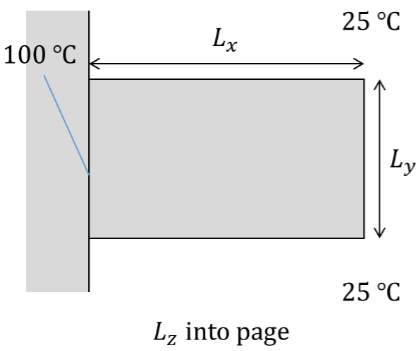
\includegraphics[width=0.3\textwidth]{fig/fin.png}
    \caption{Long Rectangular Fin Attached to Heat Source}
    \label{fig:fin}
\end{figure}

The time-dependent temperature distribution is governed by the 2D heat diffusion equation

\begin{equation}
    \pderiv{T}{t} = \alpha \left( \pderiv{^2 T}{x^2} + \pderiv{^2 T}{y^2}\right)
    \label{eq:2DHeat}
\end{equation}

where $T$ is temperature and $\alpha$ is the thermal diffusivity coefficient.\\

\textbf{Goal}: Solve Equation~\eqref{eq:2DHeat} from an initial time $t_0$ to a final time $t_f$ for the temperature distribution across the 2D rectangular fin in Figure~\ref{fig:fin} (as a function of time) using a finite-difference method.\\

The following figure shows the coordinate system and general discretization of the fin:

\begin{figure}[h]
    \centering
    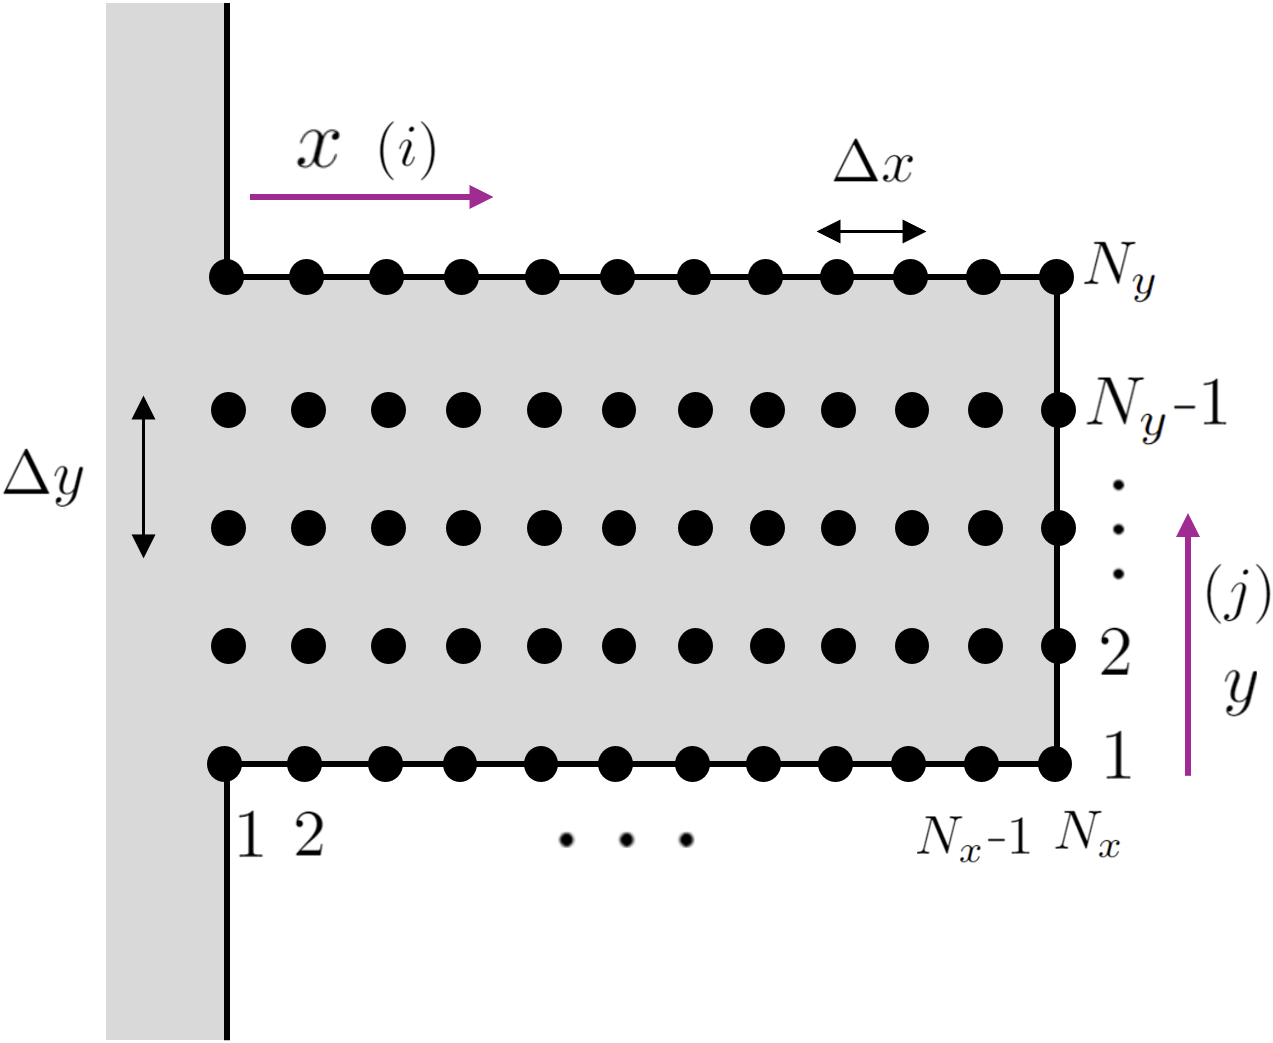
\includegraphics[width=0.45\textwidth]{fig/finSetup.png}
    \caption{Coordinate system and discretization of a 2D thin rectangular fin}
    \label{fig:finSetup}
\end{figure}

In this setup, the origin is fixed to the bottom-left corner of the fin, $\Delta x$ \& $\Delta y$ represents the node spacings, $N_x$ \& $N_y$ represents the final nodes in the $x$ \& $y$ direction, $i$ \& $j$ are the indices for the $x$ \& $y$ direction, respectively.

\pagebreak

\section{Deriving Node Equations}

In the class notes, we derived the following node equations:
\begin{align}
    \shortintertext{Interior Nodes:}
    T_{i,j}^{k+1}     & = \lambda\left(T_{i-1}^k + T_{i,j-1}^k + T_{i+1,j}^k + T_{i,j+1}^k\right) + (1-4\lambda)T_{i,j}^k                         \\
    \shortintertext{Left Boundary:}
    T_{1,j}^{k+1}     & = T_{i,j}^k = T_b \\
    \shortintertext{Right Boundary (excluding corner nodes):}
    T_{N_x,j}^{k+1}   & = \lambda\left(2T_{N_x-1,j}^k + T_{N_x,j+1}^k + T_{N_x,j-1}^k + 2BT_{\infty}\right) + (1-4\lambda - 2B\lambda)T_{N_x,j}^k \\
    \shortintertext{Top-right corner node:}
    T_{N_x,N_y}^{k+1} & = \lambda\left(2T_{N_x-1,N_y}^k + T_{N_x,N_y-1}^k + 2BT_{\infty}\right) + (1-4\lambda - 4B\lambda)T_{N_x,N_y}^k
\end{align}
where $B = \ddfrac{h \Delta x}{k}$, $\lambda = \ddfrac{\alpha \Delta t}{(\Delta x)^2}$, $\alpha = \ddfrac{k}{\rho c_p}$.\\

We must derive the remaining node equations for the top boundary, lower boundary, and the bottom-right corner:

\begin{figure}[h]
    \centering
    \subfigure[Top Nodes]{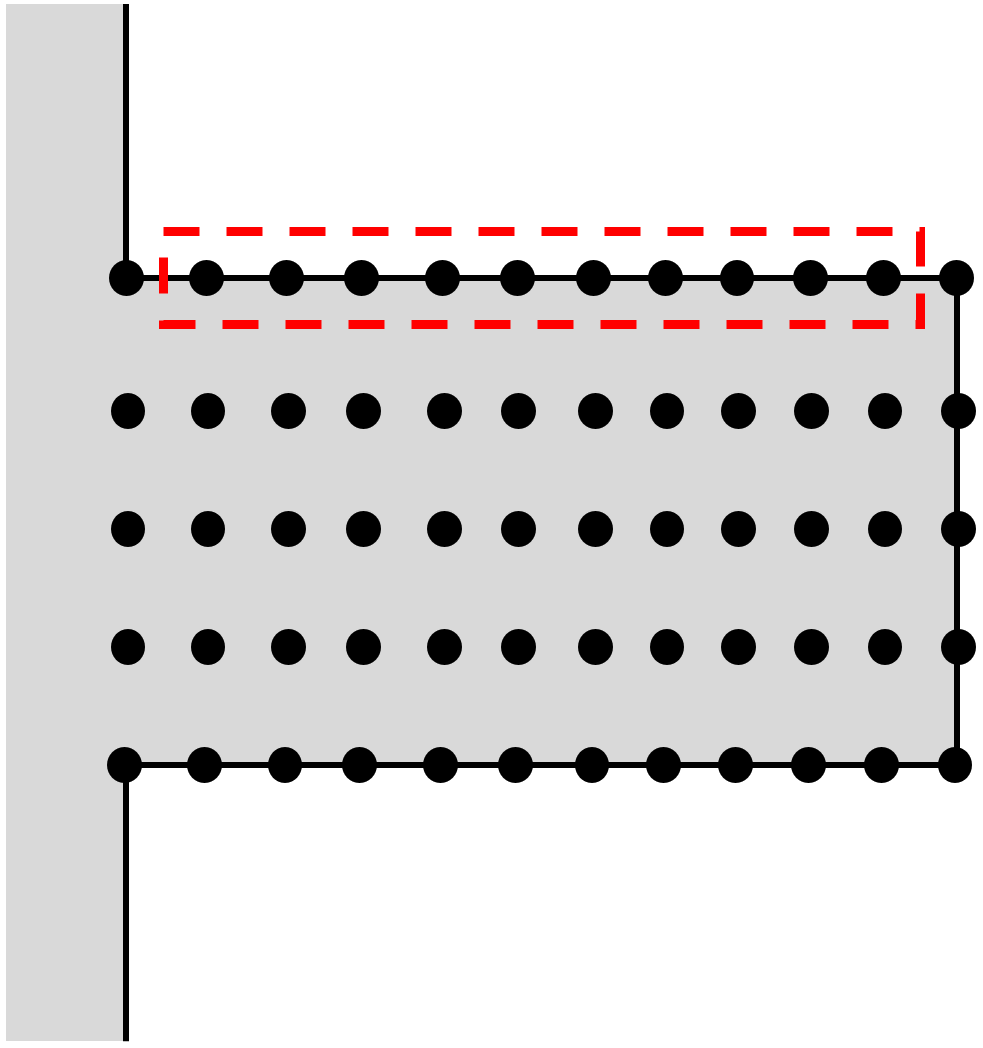
\includegraphics[width=0.24\textwidth]{fig/topNodes.png}} 
    \hspace{0.5cm}
    \subfigure[Bottom Nodes]{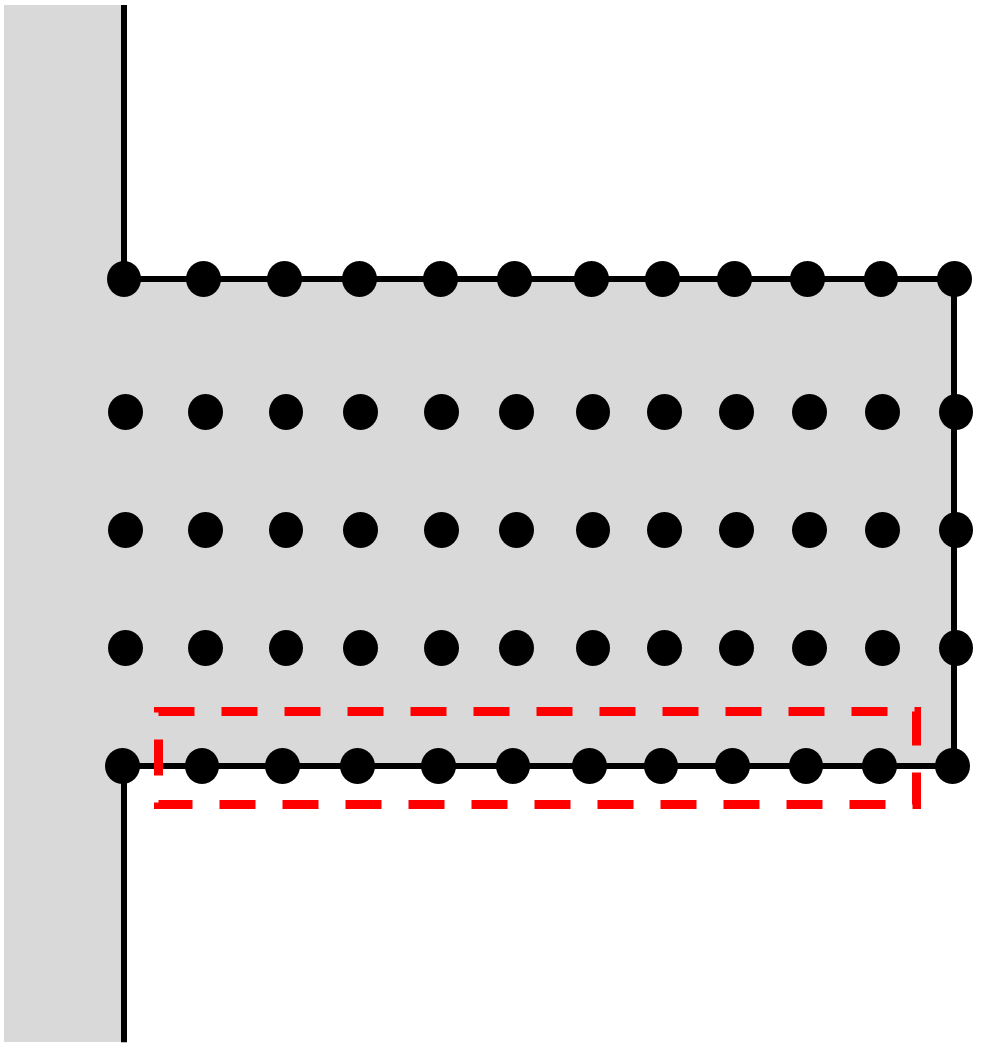
\includegraphics[width=0.24\textwidth]{fig/bottomNodes.png}} 
    \hspace{0.5cm}
    \subfigure[Corner Node]{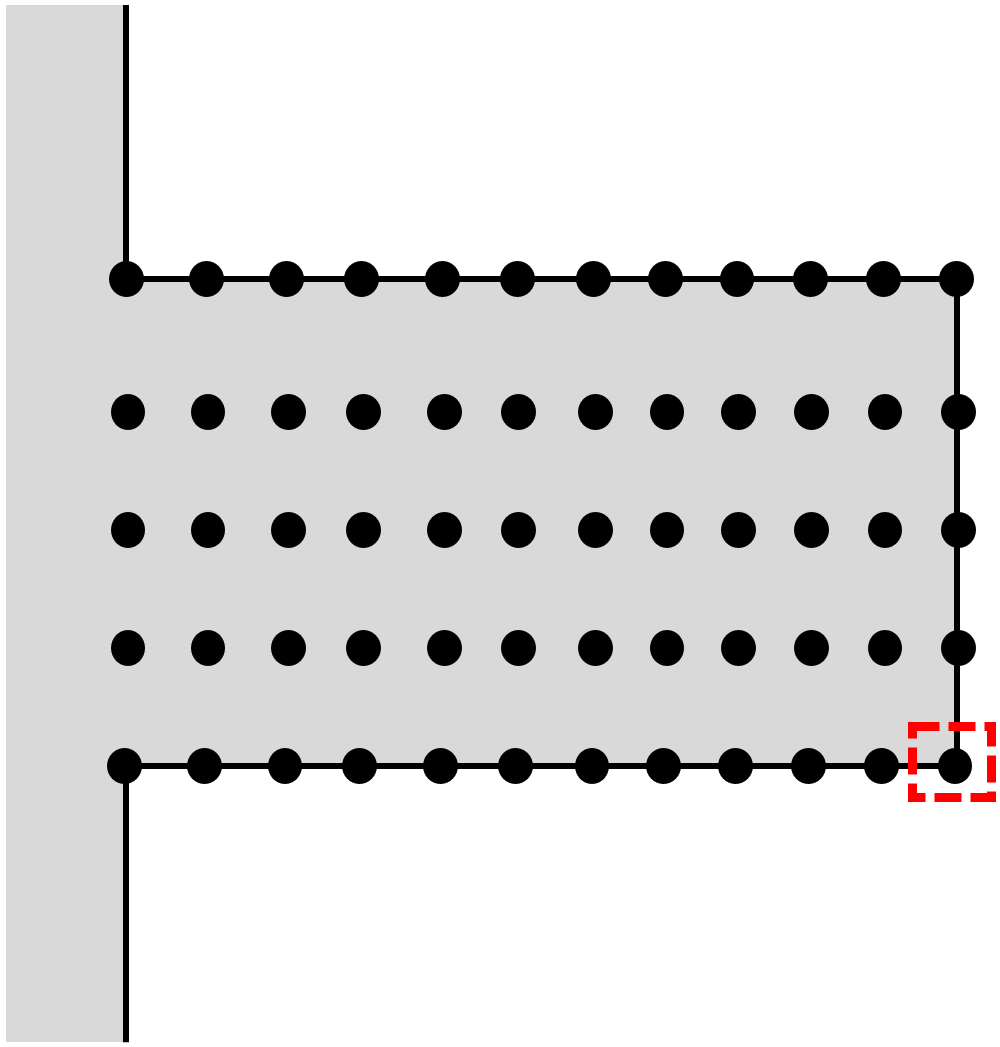
\includegraphics[width=0.24\textwidth]{fig/cornerNode.png}}
    \caption{Visualization of node configurations and boundary conditions}
    \label{fig:nodes}
\end{figure}

The energy balance at all boundary nodes is captured by:
\[
\dot{E}_{in} - \dot{E}_{out} + \dot{E}_{generated} = \dot{E}_{stored}    
\]
Since the rate of energy flowing out of the control volume is zero ($\dot{E}_{out}$) and there is no energy generation within the control volume ($\dot{E}_{generated}$ = 0), then the equation above simplifies to:
\[
\dot{E}_{in} = \dot{E}_{stored}    
\]
This implies that:
\begin{equation}
    \sum{\dot{Q}_{cond}} + \sum{\dot{Q}_{conv}} = m c_p \pderiv{T}{t}
    \label{eq:energy}
\end{equation}  
This equation represents the balance of heat energy at the node, accounting for both conductive and convective heat transfer rates and the rate of change of stored thermal energy within the fin material. For our numerical simulations, this equation can be discretized further to solve for the temperature distribution over time within the rectangular fin using finite-difference approximations.

\subsection{Top Boundary Nodes}

Consider the nodes located along the top boundary of the rectangular fin ($i$, $N_y$), excluding the corner nodes. These nodes are subject to conduction and convection with the free stream air temperature $T_{\infty}$ .\\

Using Fourier's Law of Conduction ($\dot{Q}_{cond} = kA\pderiv{T}{x}$) and Newton's Law of Cooling ($\dot{Q}_{conv} = hA\Delta T$), let's look at the flow rates coming into the control volume and their discretization:

\begin{itemize}
    \item $\dot{Q}_{cond_{1}} = kA\ddfrac{\Delta T}{\Delta y} = k(\Delta x \Delta z) \ddfrac{T_{i,1-1}^k - T_{i,1}^k}{\Delta y}$
    \item $\dot{Q}_{cond_{2}} = kA\ddfrac{\Delta T}{\Delta x} = k(\ddfrac{\Delta y}{2} \Delta z) \ddfrac{T_{i+1,N_y}^k - T_{i,1}^k}{\Delta x}$
    \item $\dot{Q}_{cond_{3}} = kA\ddfrac{\Delta T}{\Delta x} = k(\ddfrac{\Delta y}{2} \Delta z) \ddfrac{T_{i-1,N_y}^k - T_{i,1}^k}{\Delta x}$
    \item $\dot{Q}_{conv} = hA\Delta T = h(\Delta x \Delta z)\left(T_{\infty} - T_{i,1}^k\right)$
\end{itemize}

Subsituting these expressions in Equation~\eqref{eq:energy} leads to:

\begin{multline*}
    \rho\left(\Delta x \ddfrac{\Delta y}{2} \Delta z\right) c_p \ddfrac{T_{i,1}^{k+1} - T_{i,1}^k}{\Delta t} = k(\Delta x \Delta z) \ddfrac{T_{i,1-1}^k - T_{i,1}^k}{\Delta y} \\
    + k(\ddfrac{\Delta y}{2} \Delta z) \ddfrac{T_{i+1,N_y}^k - T_{i,1}^k}{\Delta x} \\
    + k(\ddfrac{\Delta y}{2} \Delta z) \ddfrac{T_{i-1,N_y}^k - T_{i,1}^k}{\Delta x}
    + h(\Delta x \Delta z)\left(T_{\infty} - T_{i,1}^k\right)
\end{multline*}

Assuming $\Delta x = \Delta y$, then this simplifies to 
\begin{center}
    \noindent \fcolorbox{red}{white}{
        $T_{i,1}^{k+1} = \lambda\left(2T_{i,1-1}^k + T_{i+1,N_y}^k + T_{i-1,N_y}^k + 2BT_{\infty}\right) + (1-4\lambda-2B\lambda)T_{i,1}^k$
        }        
\end{center}


\subsection{Lower Boundary Nodes}
Consider the nodes located along the top boundary of the rectangular fin ($i$, $1$), excluding the corner nodes. These nodes are subject to conduction and convection with the free stream air temperature $T_{\infty}$ .\\

Using Fourier's Law of Conduction and Newton's Law of Cooling, the flow rates coming into the control volume are:

\begin{itemize}
    \item $\dot{Q}_{cond_{1}} = kA\ddfrac{\Delta T}{\Delta y} = k(\Delta x \Delta z) \ddfrac{T_{i,2}^k - T_{i,1}^k}{\Delta y}$
    \item $\dot{Q}_{cond_{2}} = kA\ddfrac{\Delta T}{\Delta x} = k(\ddfrac{\Delta y}{2} \Delta z) \ddfrac{T_{i-1,1}^k - T_{i,1}^k}{\Delta x}$
    \item $\dot{Q}_{cond_{3}} = kA\ddfrac{\Delta T}{\Delta x} = k(\ddfrac{\Delta y}{2} \Delta z) \ddfrac{T_{i+1,1}^k - T_{i,1}^k}{\Delta x}$
    \item $\dot{Q}_{conv} = hA\Delta T = h(\Delta x \Delta z)\left(T_{\infty} - T_{i,1}^k\right)$
\end{itemize}

Subsituting these expressions in Equation~\eqref{eq:energy} leads to:

\begin{multline*}
    \rho\left(\Delta x \ddfrac{\Delta y}{2} \Delta z\right) c_p \ddfrac{T_{i,N_y}^{k+1} - T_{i,N_y}^k}{\Delta t} = k(\Delta x \Delta z) \ddfrac{T_{i,2}^k - T_{i,1}^k}{\Delta y} \\
    + k(\ddfrac{\Delta y}{2} \Delta z) \ddfrac{T_{i-1,1}^k - T_{i,1}^k}{\Delta x} \\
    + k(\ddfrac{\Delta y}{2} \Delta z) \ddfrac{T_{i+1,1}^k - T_{i,1}^k}{\Delta x}
    + h(\Delta x \Delta z)\left(T_{\infty} - T_{i,1}^k\right)
\end{multline*}

Assuming $\Delta x = \Delta y$, then this simplifies to 
\begin{center}
    \noindent \fcolorbox{red}{white}{
        $T_{i,1}^{k+1} = \lambda\left(2T_{i,2}^k + T_{i+1,1}^k + T_{i-1,1}^k + 2BT_{\infty}\right) + (1-4\lambda-2B\lambda)T_{i,1}^k$
        }        
\end{center}

\subsection{Bottom-right Corner Node}
Now, consider the node located on the bottom-right corner of the rectangular fin ($N_x$, $1$). This is also subject subject to conduction and convection with the free stream air temperature $T_{\infty}$ .\\

Using Fourier's Law of Conduction and Newton's Law of Cooling, the flow rates coming into the control volume are:

\begin{itemize}
    \item $\dot{Q}_{cond_{1}} = kA\ddfrac{\Delta T}{\Delta x} = k(\ddfrac{\Delta y}{2} \Delta z) \ddfrac{T_{N_x-1,1}^k - T_{N_x,1}^k}{\Delta x}$
    \item $\dot{Q}_{cond_{2}} = kA\ddfrac{\Delta T}{\Delta y} = k(\ddfrac{\Delta x}{2} \Delta z) \ddfrac{T_{N_x,2}^k - T_{N_x,1}^k}{\Delta y}$
    \item $\dot{Q}_{conv_{1}} = hA\Delta T = h(\ddfrac{\Delta x}{2} \Delta z) \left(T_{\infty} - T_{N_x,1}^k\right)$
    \item $\dot{Q}_{conv_{2}} = hA\Delta T = h(\ddfrac{\Delta y}{2} \Delta z)\left(T_{\infty} - T_{N_x,1}^k\right)$
\end{itemize}

Subsituting these expressions in Equation~\eqref{eq:energy} leads to:

\begin{multline*}
    \rho\left(\ddfrac{\Delta x}{2} \ddfrac{\Delta y}{2} \Delta z\right) c_p \ddfrac{T_{N_x,1}^{k+1} - T_{N_x,1}^k}{\Delta t} = k(\ddfrac{\Delta y}{2} \Delta z) \ddfrac{T_{N_x-1,1}^k - T_{N_x,1}^k}{\Delta x} \\
    + k(\ddfrac{\Delta x}{2} \Delta z) \ddfrac{T_{N_x,2}^k - T_{N_x,1}^k}{\Delta y} \\
    + h(\ddfrac{\Delta x}{2} \Delta z) \left(T_{\infty} - T_{N_x,1}^k\right)
    + h(\ddfrac{\Delta y}{2} \Delta z)\left(T_{\infty} - T_{N_x,1}^k\right)
\end{multline*}

Assuming $\Delta x = \Delta y$, then this simplifies to 
\begin{center}
    \noindent \fcolorbox{red}{white}{
        $T_{N_x,1}^{k+1} = 2\lambda\left(T_{N_x-1,1}^k + T_{N_x,2}^k + 2BT_{\infty}\right) + (1-4\lambda-4B\lambda)T_{N_x,1}^k$
        }        
\end{center}

\pagebreak

\section{Scenarios}

Let's analyze each scenario based on the values of thermal conductivity ($k_{\textrm{cond}}$), thermal diffusivity ($\alpha$), and convection coefficient ($h$) listed in the table below:

\begin{table}[h]
    \centering
    \caption{Five Scenarios Using an Explicit Finite-Difference Method}
    \small
    \begin{threeparttable}
        \begin{tabular}{|s|c|c|c|c|c|c|c|c|} \hline
            {\cellcolor{yellow!50} \bf Scenario} & {\PB{1cm}{$k_{\textrm{cond}}$                                                                 \\$\left(\frac{\textrm{W}}{\textrm{m} \, {}^{\circ}\textrm{C}}\right)$}} & {\PB{1.2cm}{$\alpha$\\$\left(\frac{\textrm{m}^2}{\textrm{s}}\right)$}} & {\PB{1.1cm}{$h$\\$\left(\frac{\textrm{W}}{\textrm{m}^2 \, {}^{\circ}\textrm{C}}\right)$}} & {\PB{0.8cm}{$t_{ss}$\\(min)}} & {\PB{1.3cm}{$T_{\textrm{avg}}$ tip\\1D eqn* (${}^{\circ}$C)}} &  {\PB{1.3cm}{$T_{\textrm{avg}}$ tip\\sim* (${}^{\circ}$C)}} & {\PB{1.3cm}{$\dot{Q}$\\1D eqn* (W)}} & {\PB{1.3cm}{$\dot{Q}$\\sim* (W)}}
            \\ \hline
            Pure Al, fan high                    & 240                           & \SI{97e-6}{}  & 100 & 0.93  & 93.94 & 94.16 & 133.31 & 126.32 \\ \hline
            Pure Al, fan low                     & 240                           & \SI{97e-6}{}  & 10  & 0.99  & 99.35 & 99.37 & 14.02  & 13.27  \\ \hline
            AISI 302                             & 15                            & \SI{4e-6}{}   & 100 & 11.23 & 52.54 & 53.57 & 78.49  & 74.32  \\ \hline
            Low $k$, high $\alpha$               & 3                             & \SI{100e-6}{} & 100 & 0.055 & 28.77 & 29.40 & 37.61  & 34.43  \\ \hline
            High $k$, low $\alpha$               & 100                           & \SI{3e-6}{}   & 100 & 27.51 & 86.72 & 87.18 & 124.08 & 117.68 \\  \hline
        \end{tabular}
        \label{tab:Scenarios}
        \begin{tablenotes}
            \item [*] The average tip temperature and heat rate are the values at the end of the simulation, which are well past the time when the contour lines stop moving.
        \end{tablenotes}
    \end{threeparttable}
\end{table}

We'll first look at case 1 (Pure Al, fan high), and then show how adjusting these parameters affects the temperature distribution, time to reach steady-state, and heat rate into the fin for scenarios 2-5.

\pagebreak

\subsection{Scenario 1: Pure Aluminum, Fan High}

\begin{figure}[h]
    \centering
    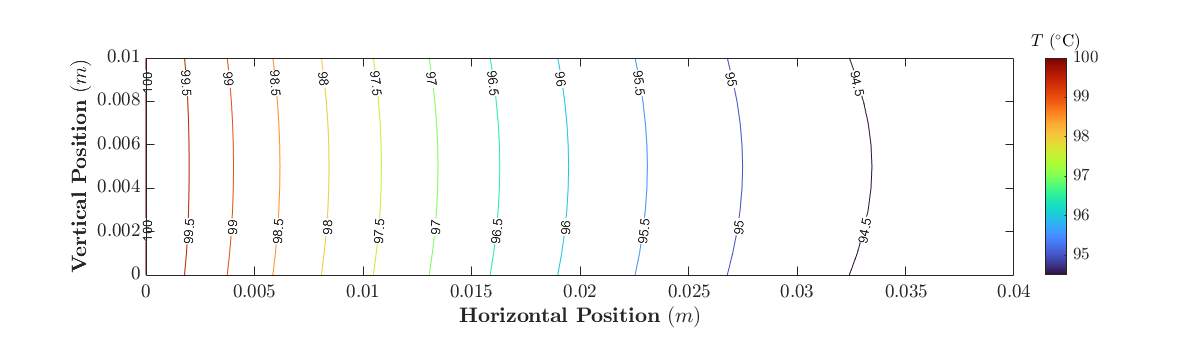
\includegraphics[width=1\textwidth]{fig/contour1.png}
    \caption{Steady-State Temperature Distrubution for Scenario 1}
    \label{fig: Plot1}
\end{figure}

Simulation Parameters:
\begin{itemize}
    \item d$t$ = 0.0012
    \item $N_t$ = 500,000
    \item $B$ = $\SI{4.167e-4}{}$
    \item $\lambda$ = 0.1164
\end{itemize}

\pagebreak

\subsection{Scenario 2: Pure Aluminum, Fan Low}

\begin{figure}[h]
    \centering
    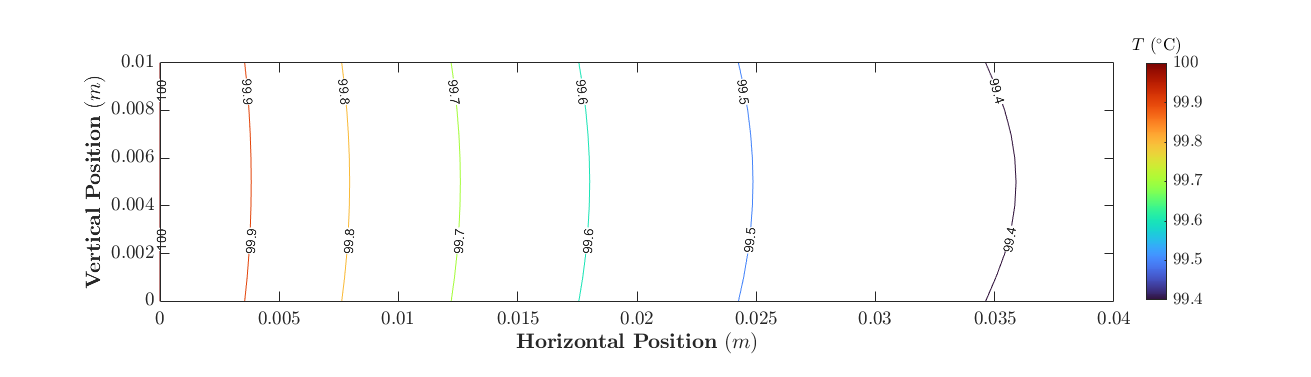
\includegraphics[width=1\textwidth]{fig/contour2.png}
    \caption{Steady-State Temperature Distrubution for Scenario 2}
    \label{fig: Plot2}
\end{figure}

Simulation Parameters:
\begin{itemize}
    \item d$t$ = 0.00015
    \item $N_t$ = 200,000
    \item $B$ = $\SI{4.167e-4}{}$
    \item $\lambda$ = 0.1455
\end{itemize}

Effect of Adjustments:
\begin{itemize}
    \item \textbf{Temperature Distrubution}:
    \item \textbf{Time to Steady State ($t_{ss}$)}:
    \item \textbf{Heat Rate ($\dot{Q}$)}:
\end{itemize}

\pagebreak

\subsection{Scenario 3: Stainless Steel, AISI 302}

\begin{figure}[h]
    \centering
    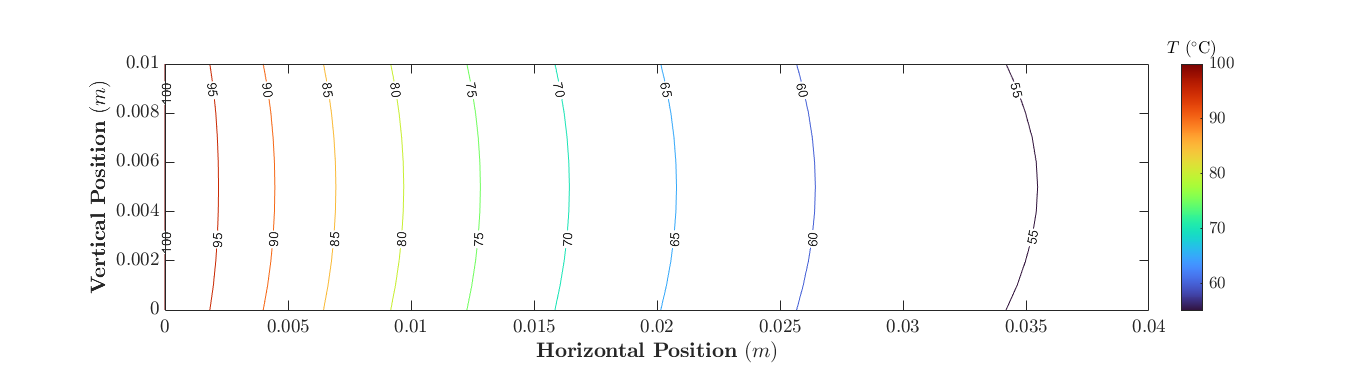
\includegraphics[width=1\textwidth]{fig/contour3.png}
    \caption{Steady-State Temperature Distrubution for Scenario 3}
    \label{fig: Plot3}
\end{figure}

Simulation Parameters:
\begin{itemize}
    \item d$t$ = 0.0015
    \item $N_t$ = 100,000
    \item $B$ = $\SI{6.667e-3}{}$
    \item $\lambda$ = 0.06
\end{itemize}

Effect of Adjustments:
\begin{itemize}
    \item \textbf{Temperature Distrubution}:
    \item \textbf{Time to Steady State ($t_{ss}$)}:
    \item \textbf{Heat Rate ($\dot{Q}$)}:
\end{itemize}

\pagebreak

\subsection{Scenario 4: Low $k$, high $\alpha$}

\begin{figure}[h]
    \centering
    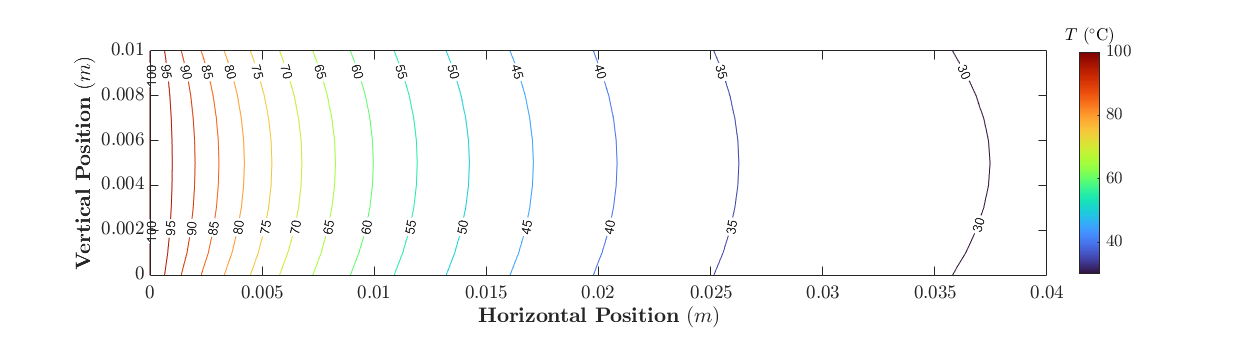
\includegraphics[width=1\textwidth]{fig/contour4.png}
    \caption{Steady-State Temperature Distrubution for Scenario 4}
    \label{fig: Plot4}
\end{figure}

Simulation Parameters:
\begin{itemize}
    \item d$t$ = 0.0015
    \item $N_t$ = 200,000
    \item $B$ = $\SI{0.0333}{}$
    \item $\lambda$ = 0.15
\end{itemize}

Effect of Adjustments:
\begin{itemize}
    \item \textbf{Temperature Distrubution}:
    \item \textbf{Time to Steady State ($t_{ss}$)}:
    \item \textbf{Heat Rate ($\dot{Q}$)}:
\end{itemize}

\pagebreak

\subsection{Scenario 5: High $k$, low $\alpha$}

\begin{figure}[h]
    \centering
    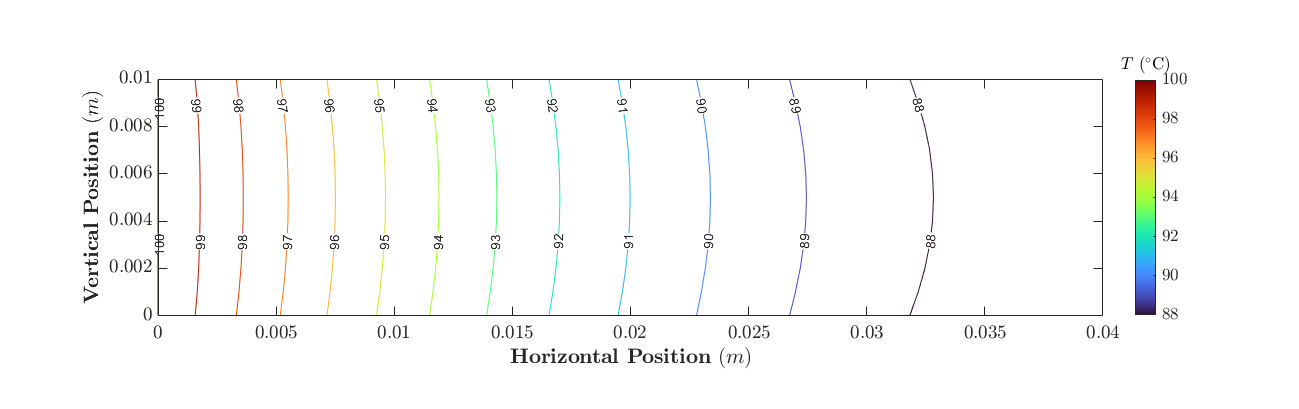
\includegraphics[width=1\textwidth]{fig/contour5.png}
    \caption{Steady-State Temperature Distrubution for Scenario 5}s
    \label{fig: Plot5}
\end{figure}

Simulation Parameters:
\begin{itemize}
    \item d$t$ = 0.0120
    \item $N_t$ = 200,000
    \item $B$ = 0.036
    \item $\lambda$ = 0.01
\end{itemize}

Effect of Adjustments:
\begin{itemize}
    \item \textbf{Temperature Distrubution}:
    \item \textbf{Time to Steady State ($t_{ss}$)}:
    \item \textbf{Heat Rate ($\dot{Q}$)}:
\end{itemize}

\end{document}
